\documentclass{homework}

\title{Homework 10}
\author{Kevin Evans}
\studentid{11571810}
\date{April 12, 2020}
\setclass{Physics}{304}
\usepackage{amssymb}
\usepackage{mathtools}

\usepackage{amsthm}
\usepackage{amsmath}
\usepackage{slashed}
\usepackage{relsize}
\usepackage{threeparttable}
\usepackage{float}
\usepackage{booktabs}
\usepackage{boldline}
\usepackage{changepage}
\usepackage{physics}
\usepackage[inter-unit-product =\cdot]{siunitx}
\usepackage{setspace}

\usepackage[makeroom]{cancel}
\usepackage{pgfplots}

\usepackage{multicol}
\usepackage{tcolorbox}
\usepackage{enumitem}
\usepackage{times}
\usepackage{mhchem}
\usepackage{graphicx} 
\DeclareSIUnit{\year}{yr}
\usepackage[export]{adjustbox}

\begin{document}
	\maketitle
	\subsubsection*{Chapter 12 (B)}
	\begin{enumerate}[label={\arabic*.}]%[label=\textbf{Problem {\arabic*.}}, align=left]
		\item At $T=0$, a metal with a half-filled band can still conduct as an external electric field is being applied. The electric field ``gives'' some energy to the electrons, allowing them to flow.
		
		\item When a photon is absorbed, an electron is excited from the valance band to the conduction band with that photon's energy and a hole is created in the valance band. 
		
		\item \begin{enumerate}
			\item If the gap is \SI{1.14}{\eV}, the photon would have that same energy, \begin{align*}
					f & = E / h \\
						& = \frac{ \SI{1.14}{\eV} }{ \SI{4.135e-15}{\eV \s} } \\
						& = \SI{2.75e14}{\Hz}
			\end{align*}
			\item For the wavelength for that photon, \begin{align*}
				f\lambda & = c \\
				\lambda & =  c / f = \frac{\SI{3e8}{\m\per\s}}{\SI{2.75e14}{\Hz}} \\
					& = \SI{1.1}{\um} \quad \text{(near-infrared)}
			\end{align*}
		\end{enumerate}
	
		\item The light is absorbed by electrons in silicon with energies that exceed the minimum energy (the gap energy). In diamond, the light is able to pass without absorption since the light does not have enough energy to excite electrons from the valance band. 
		
		\item For wavelengths under \SI{1}{\um}, the maximum energy from those photons would be \SI{1.24}{\eV}. Probably the germanium would be a better choice, as the energy required is much less than silicon, and lower energy photons would have a higher chance of exciting electrons in germanium.
		
		\item For the energy gap of \SI{5.5}{\eV}, the photons corresponding to that energy would have a wavelength \begin{align*}
			\lambda & = \frac{c}{f} = \frac{hc}{E} \\
				& = \frac{\SI{1240}{\eV \nm}}{\SI{5.5}{\eV}} = \SI{225}{\nm}
		\end{align*}
		At wavelengths shorter than that, the energy would exceed \SI{5.5}{\eV} and would allow the absorption of photons by valance electrons.
		
		\item Sample A is a semiconductor.
			
			Sample B is a conductor.
			
			In semiconductors, more electrons are held within the conduction band as the temperature increases. 
			
		\item  \begin{enumerate}
			\item In a $p$-type semiconductor, the Fermi energy is lowered at a level near the upper edge of the valance band. This is since the semiconductor is doped with trivalant atoms. 
			\item In $n$-type semiconductors, the Fermi level is raised near the conduction band. The doped atoms donate additional electrons, lowering the energy gap required for electrons to populate the conduction band.
		\end{enumerate}
	
		\item \begin{enumerate}
			\item At the junction boundary (the depletion zone), some electrons from the $n$-type material will move into the holes in the $p$-type semiconductor, as it's more energetically favorable. This will create a potential difference at the junction.
			
			Additionally, the levels will shift, such that the Fermi levels are at an equal level on both sides.
			
			\item The electrons will move right, from the $n$-type to the $p$-type.
			
			\item The $p$-type will move up and the $n$-type will move down, until a point where the Fermi levels are equal on both sides. 
		\end{enumerate}
	
	\item 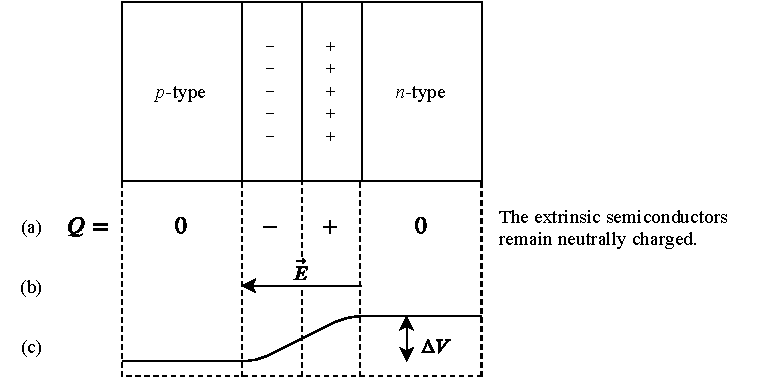
\includegraphics[valign=t]{hw10pn}
	\end{enumerate}
\end{document}